%\documentclass{article}
%\usepackage{fixltx2e}
%\usepackage{caption}
%\usepackage{graphicx}
%\begin{document}
\begin{figure}
\begin{minipage}{0.60\textwidth}
  \centering
  
	\begin{center}
	\begin{tabular}{ |c| } 
 	\hline
 		Frequent Items\\ \hline\hline
 		a \\ \hline
 		b \\ \hline
 		c \\ \hline
 		d \\ \hline
 		dc \\ \hline
 		da \\ \hline
 		dca \\ \hline
 		ca \\ \hline
\end{tabular}
\end{center}  
  
  
  \captionof{table}{\emph{Frequent Items}\\(with false positive)}
\end{minipage}
\hfill
\begin{minipage}{0.40\textwidth}
  \centering
  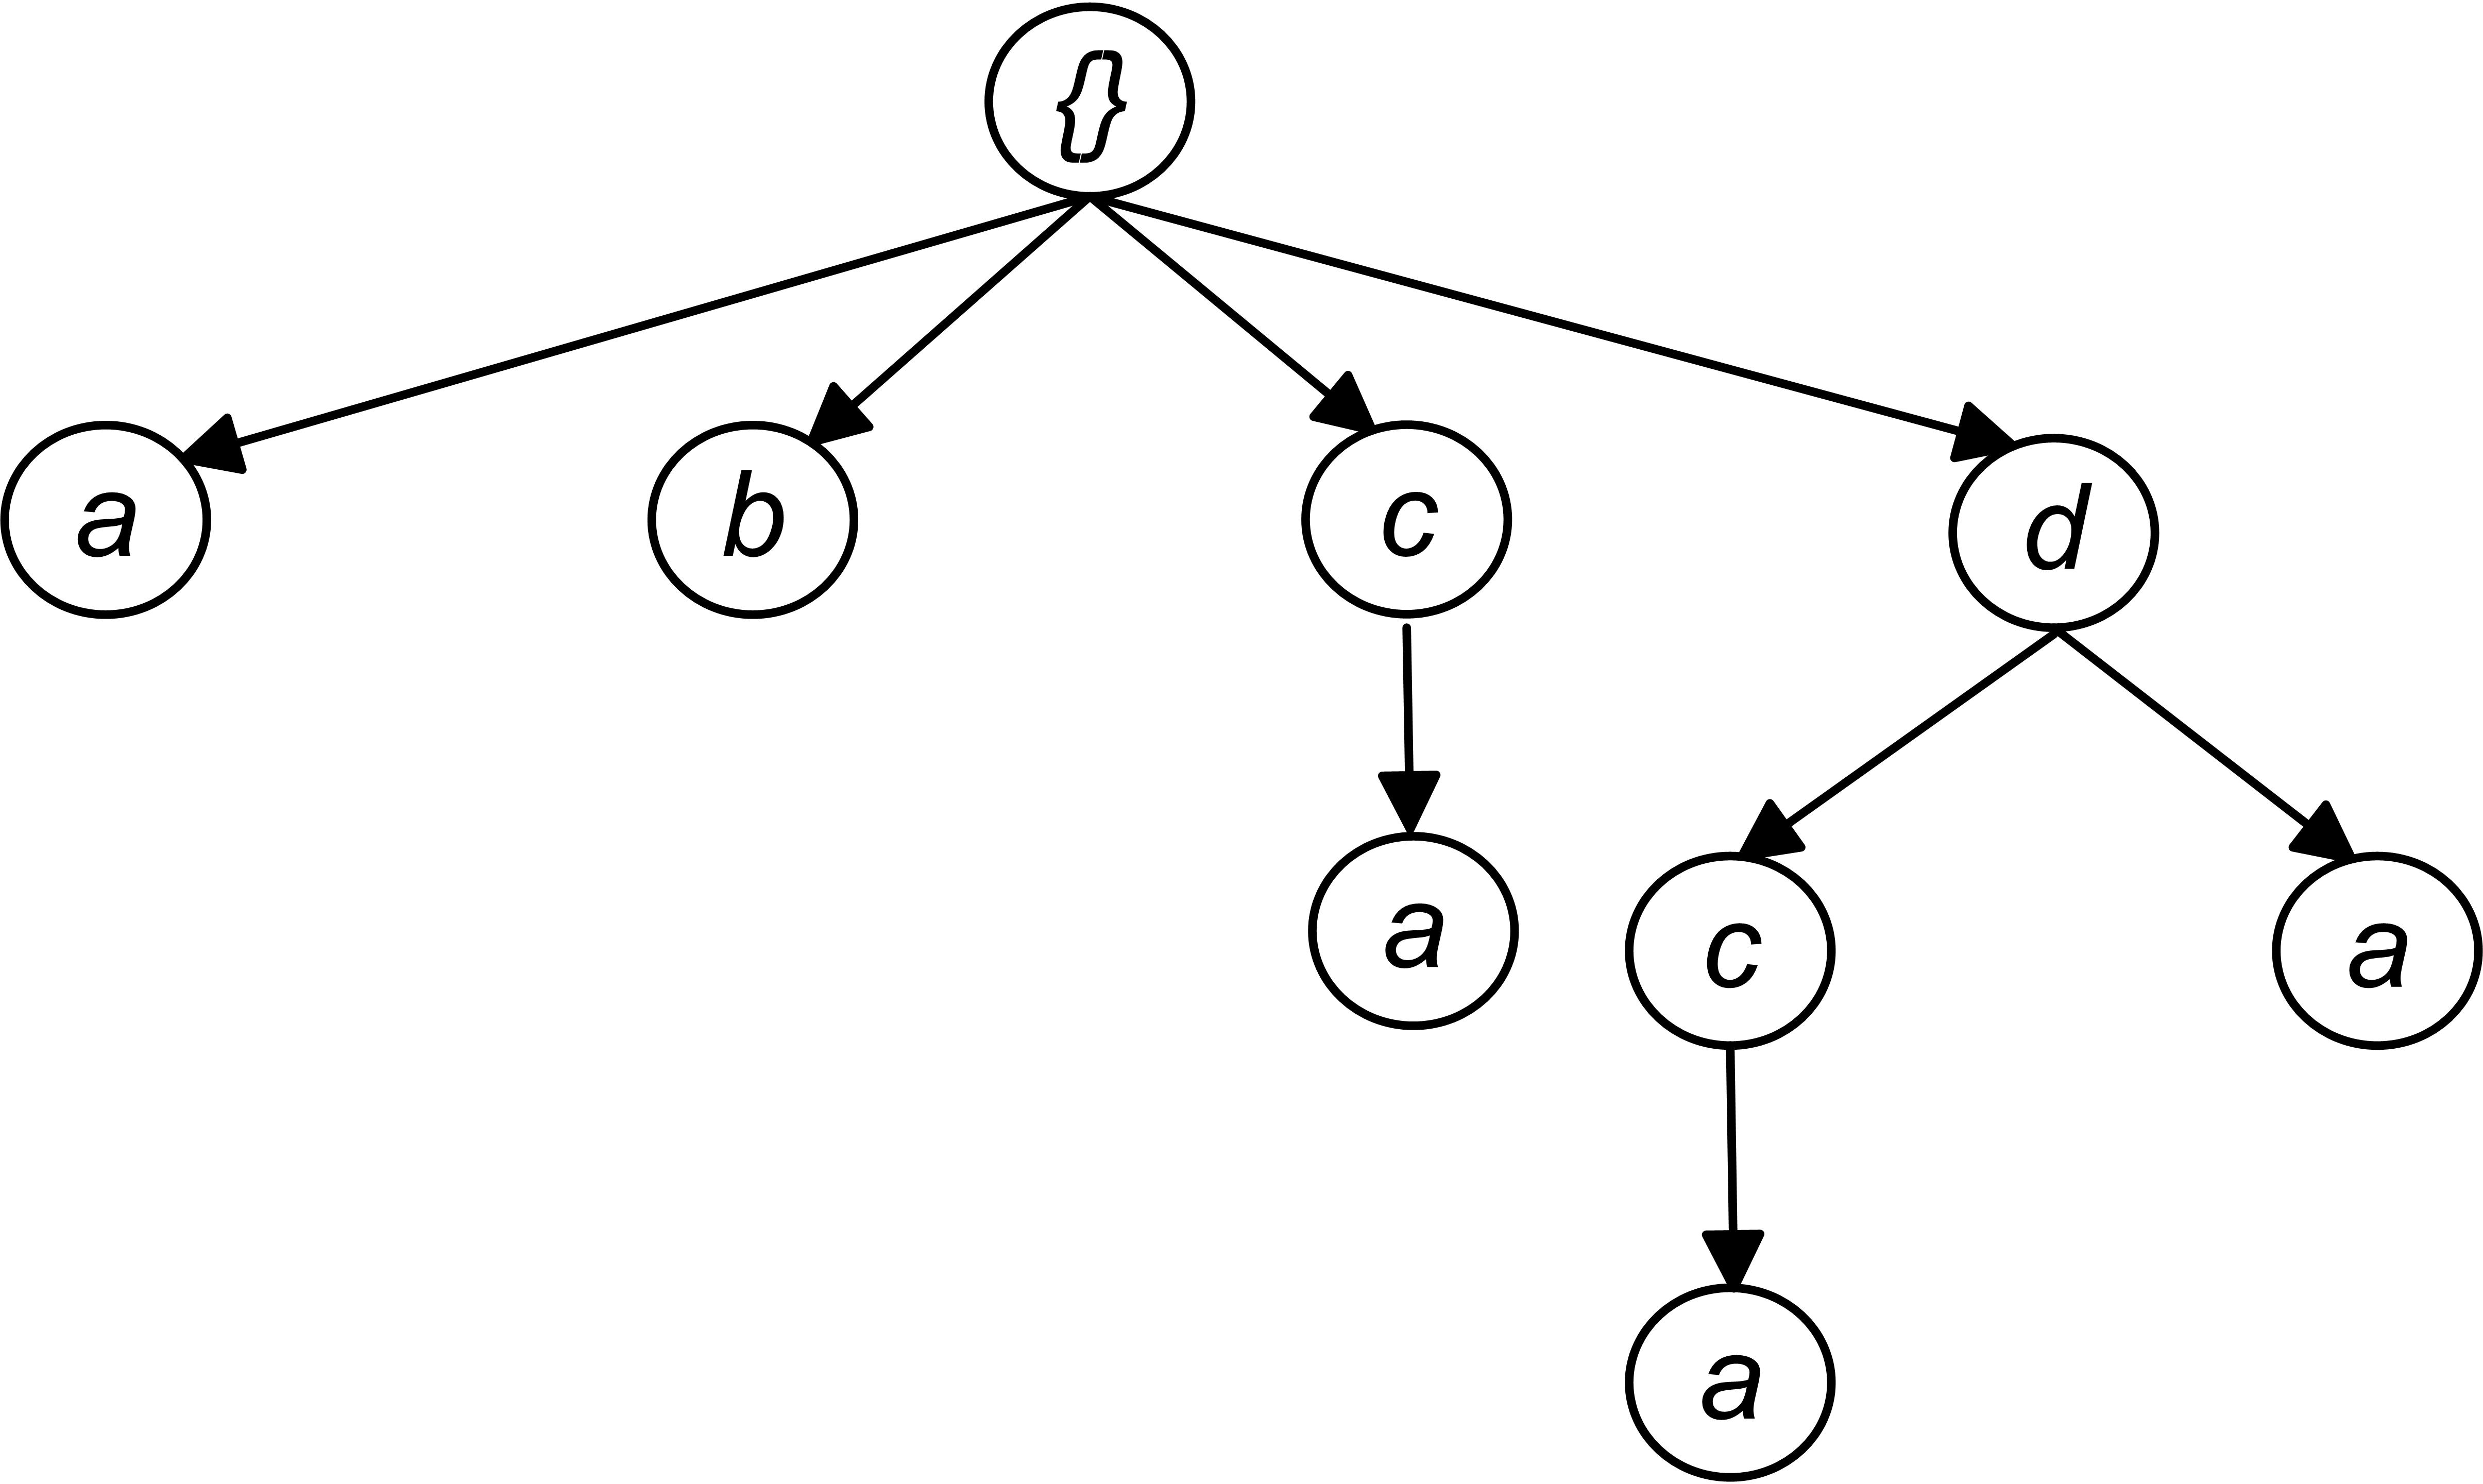
\includegraphics[width=\textwidth]{../images/frequent_tree.jpg}
  \captionof{figure}{\emph{Frequent Item Tree} }
\end{minipage}
\end{figure}
\begin{figure}
\begin{minipage}{.6\textwidth}
  \centering
  
	\begin{center}
	\begin{tabular}{ |c|c| } 
 	\hline
 		No & Items \\ \hline\hline
 		a  & \emph{a(0.9),c(0.6),d(0.5)}\\ \hline
 		b & \emph{a(0.9),b(0.4),e(0.1)}\\ \hline
 		c & \emph{a(0.2),c(0.9),d(0.7)}\\ \hline
 		d & \emph{b(0.3),c(0.9)}\\ \hline
 		dc& \emph{a(0.1),b(0.3),c(0.9)} \\ \hline
 		da & \emph{a(0.9),e(0.3)
}\\ \hline
\end{tabular}
\end{center}  
  
  
  \captionof{table}{Transaction Table after removing Infrequent Items}
\end{minipage}
\hfill
\begin{minipage}{0.40\textwidth}
  \centering
  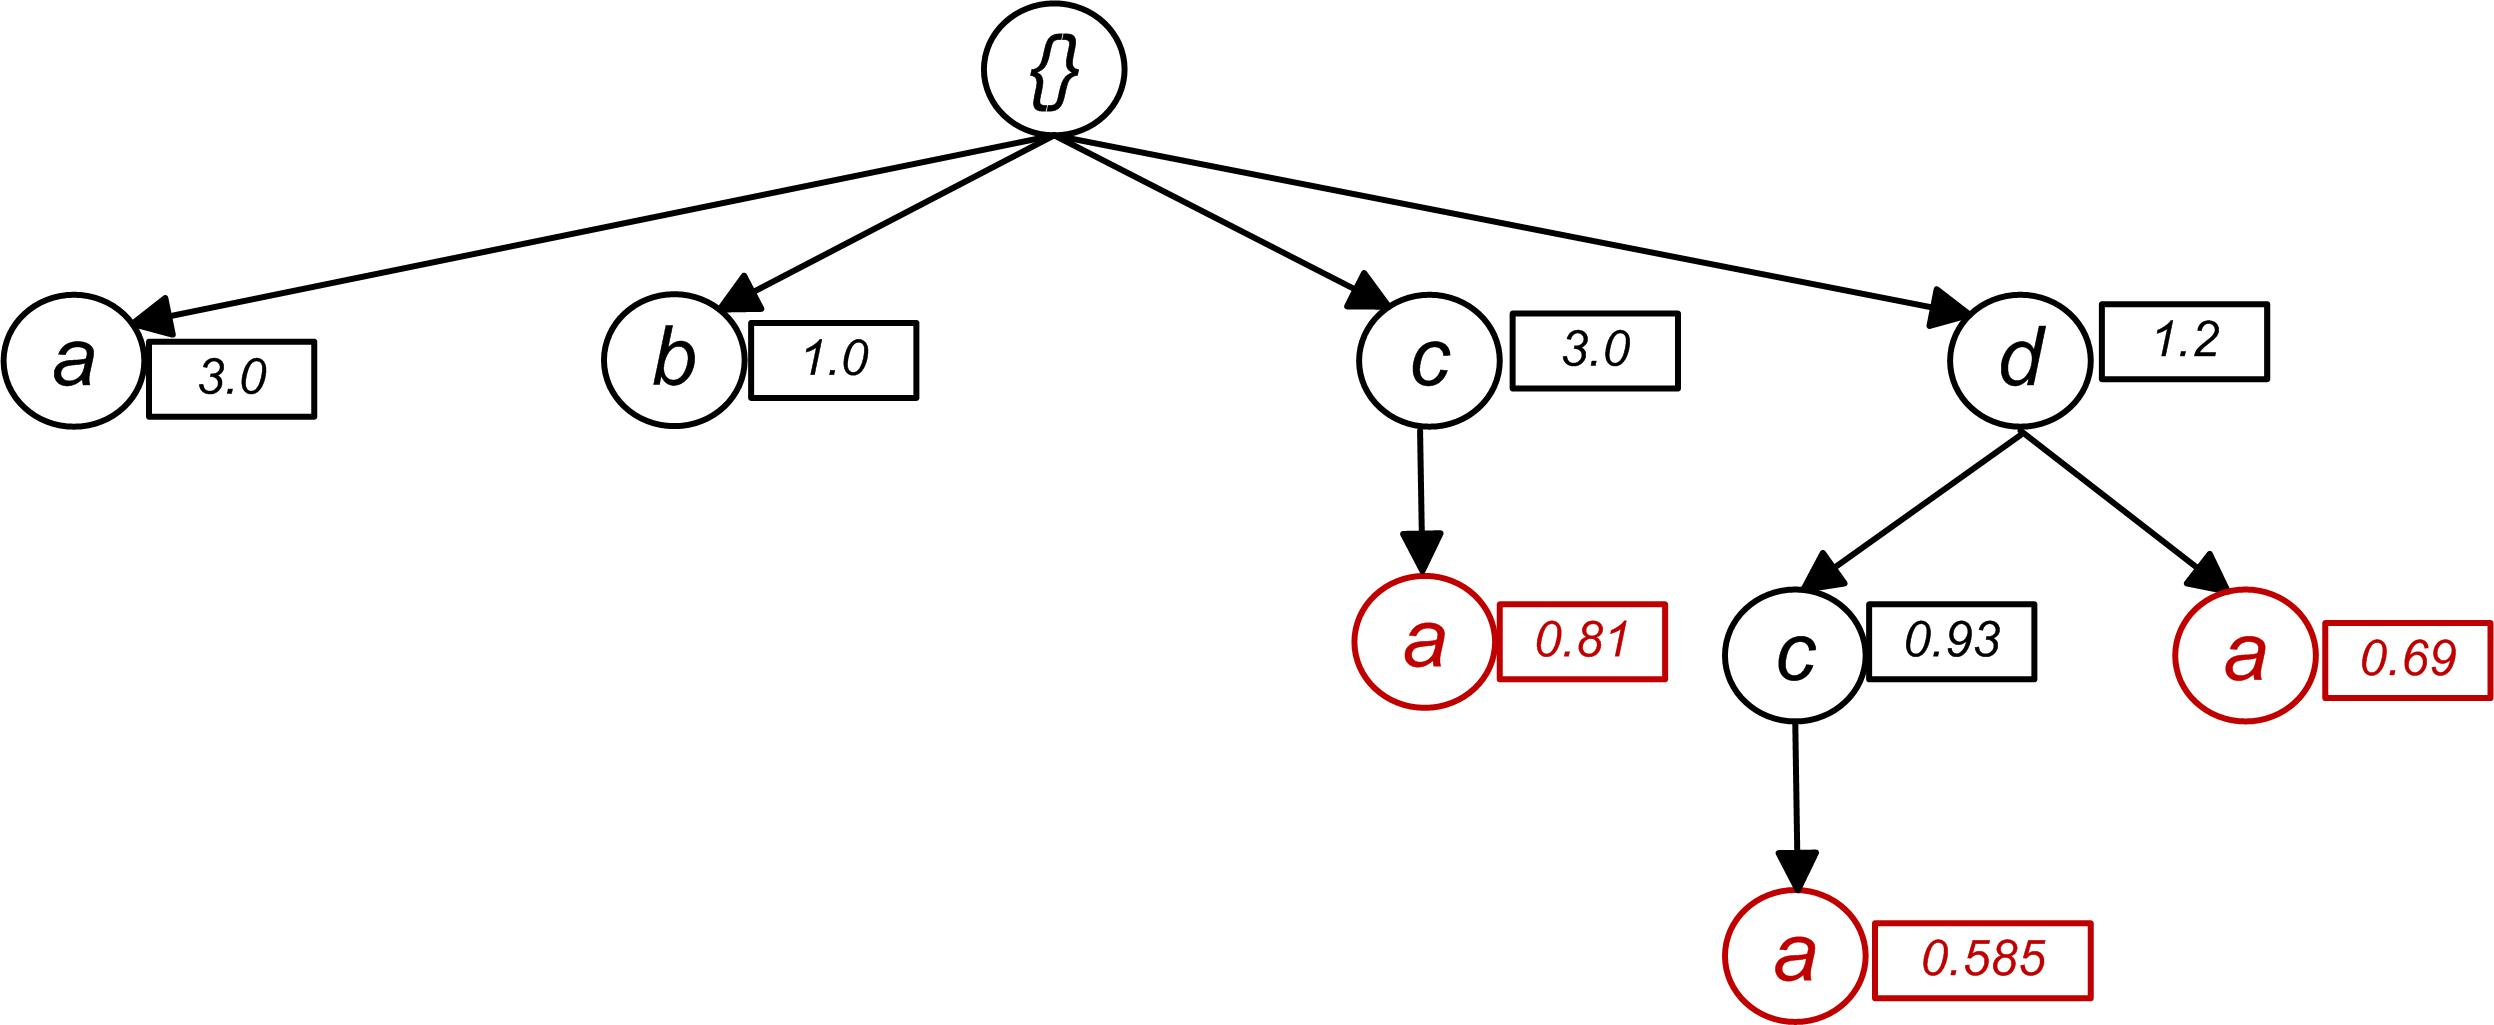
\includegraphics[width=.8\textwidth]{../images/frequent_tree_final.jpg}
  \captionof{figure}{\emph{Frequent Item Tree} identifying false positives}
\end{minipage}

\end{figure}
%\end{document}
